\section{Design Choices}
\subsection{Choice of Embedded DSL approach}

\begin{frame}{Microclassification of DSLs}
\begin{figure}[H]
  \centering
    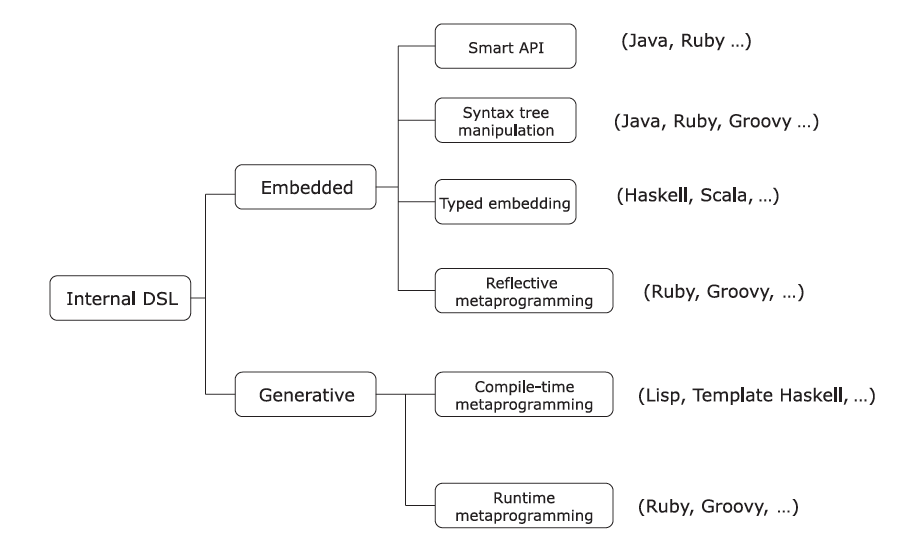
\includegraphics[width=280px]{figures/classification.png}
  \caption{Classification of DSLs}
\end{figure}
\end{frame}

\begin{frame}{Choice of Embedded DSL approach}
\begin{itemize}
\item Lightweight
\item Compile Time Type Checking
\item Easily maintainable and extensible
\item Emphasis on Semantics
\item Loose Coupling
\item Representational Independence
\end{itemize}
\begin{figure}[H]
  \centering
    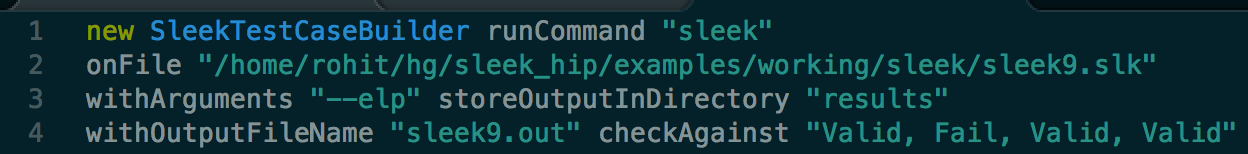
\includegraphics[width=320px]{figures/declarative_syntax.png}
  \caption{Meaningful Semantics}
\end{figure}
\end{frame}

\subsection{Choice of Programming Language}
\begin{frame}{Choice of Programming Language}
\begin{figure}[h!]
%   \centering
    
\includegraphics[height=30px]{figures/scala-logo.png}
    \
    \
    
\includegraphics[height=30px]{figures/python_lang.png}
\end{figure}
\end{frame}

% \subsection{Comparison of Scala and Python for DSL implementation}
% \begin{frame}{Advantages of Python}
% \begin{itemize}
% \item Dynamic Language
% \item Support for scripting
% \item Lower development time
% \item Easier to learn \cite{lund}
% \end{itemize}
% \begin{figure}[H]
%   \centering
%     
\includegraphics[width=150px]{figures/python_lang.png}
%   \caption{Python}
% \end{figure}
% \end{frame}

\begin{frame}{Reasons for choosing Scala}
\begin{figure}[H]
  \centering
    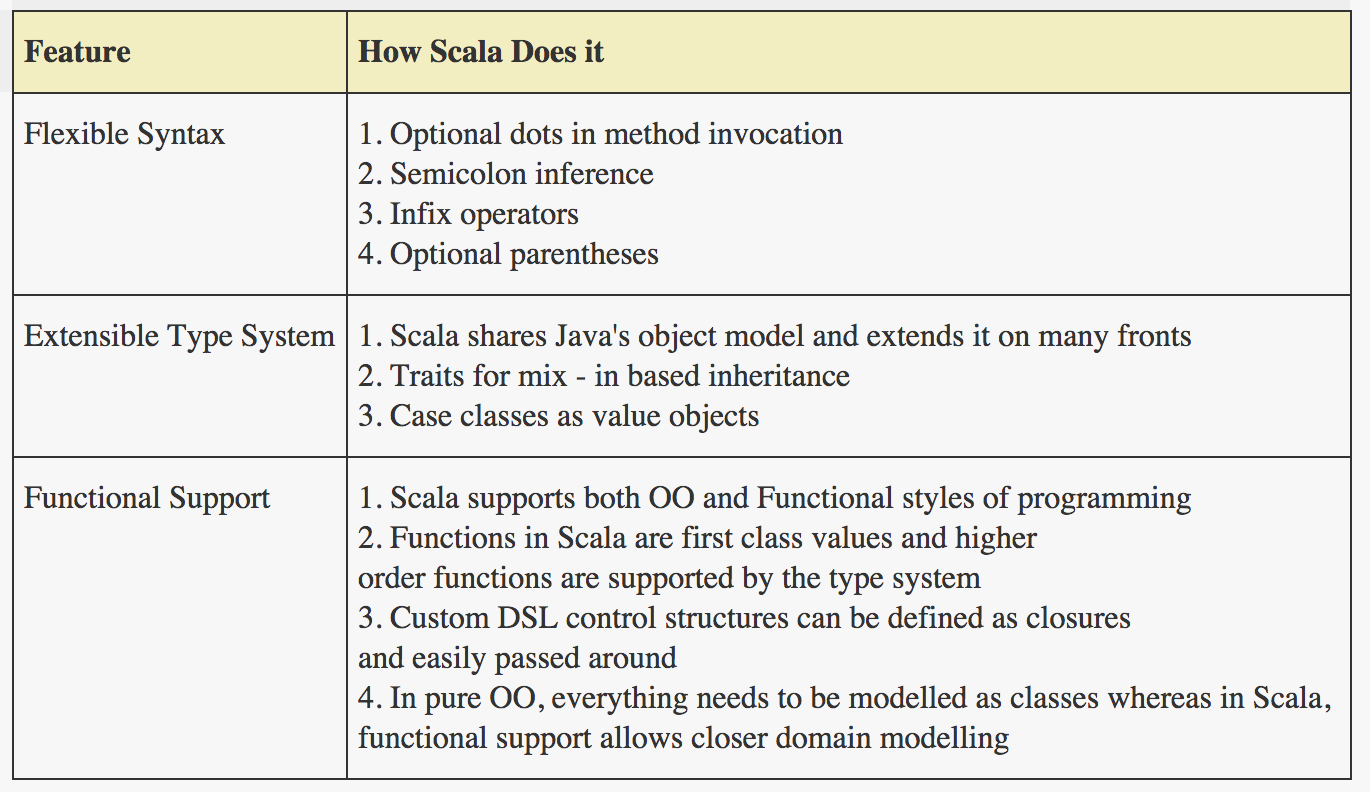
\includegraphics[width=300px]{figures/scala_motivation.png}
  \caption{Motivation for using Scala}
\end{figure}
\end{frame}

\begin{frame}{Scala is a better choice}
\begin{itemize}
\item Greater type safety due to compile time checking \cite{dslsInAction}
\item Better collections hierarchy
\item Expressiveness
\item High readability
\item Flexible Syntax
\item Functional Programming Support
\end{itemize}
\end{frame}

% \begin{frame}{Scala is a better choice}
% The DSL for repository testing was written in both Python and Scala for comparison purposes and it was concluded that Scala was a better choice for DSL development.
% \bigskip
% \noindent
% Overall, \textbf{Scala} was concluded to be more suitable for DSL development. The primary reason for this was \textit{type - safety}. DSLs can grow to several tens of thousands of lines of code and type - safety makes development a lot more robust and secure.
% \end{frame}

